\documentclass[11pt,a4paper]{report}

% House rule: no en or em dashes anywhere, and never a literal double hyphen in
% prose. Enforced by scripts/check_no_dashes.py as the last build step.

\usepackage[utf8]{inputenc}
\usepackage[T1]{fontenc}
\usepackage{lmodern}
\usepackage[margin=1in]{geometry}
\usepackage{graphicx}
\graphicspath{{figures/}}
\usepackage{amsmath}
\usepackage{booktabs}
\usepackage{siunitx}
\usepackage{caption}
\usepackage[hidelinks]{hyperref}
\usepackage{xcolor}

\title{Measuring What Spec Sheets Only Claim:\\
Cache Latency, STREAM Bandwidth, and Peak SIMD FLOPS\\
on an Intel Core i7-14700K}
\author{Olajide Badejo}
\date{July 2026}

\begin{document}

\maketitle

\begin{abstract}
This report measures, on real hardware, the numbers usually quoted from
specification sheets: cache load use latencies, sustainable memory bandwidth,
and peak single precision floating point throughput. Every figure is measured
on an Intel Core i7-14700K running inside WSL2, using timing and known transfer
sizes rather than hardware performance counters, which WSL2 does not expose. A
prefetcher defeating pointer chase recovers the L1, L2, L3, and DRAM plateaus
and cross checks them against sysfs. STREAM in three variants gives a bandwidth
scaling curve that saturates well before the cores do. A ten chain FMA loop
reaches the peak throughput computed from a software measured clock, to within
one percent. The ceilings are assembled into a measured roofline, and a BLIS
style analytical tile prediction is validated against a blocked GEMM sweep. The
prediction misses the naive kernel by design, and that miss is reported as a
finding rather than hidden.
\end{abstract}

\tableofcontents

\chapter{Introduction}

Specification sheets quote cache latencies in cycles, memory bandwidth in
gigabytes per second, and peak floating point throughput in GFLOPS. These
numbers are ceilings under idealized assumptions. What a program actually sees
depends on the access pattern, the compiler, the memory hierarchy under load,
and the clock the core really runs at. This project measures those numbers
directly on one machine, an Intel Core i7-14700K, and assembles them into a
model that predicts something concrete: the cache block sizes a blocked matrix
multiply should use.

The work has five measured pillars. First, a dependent load pointer chase
recovers the load use latency of each cache level, from a 4 KB working set that
lives in L1 up to a 512 MB working set that is firmly in DRAM, and a change
point detector locates the plateau boundaries and cross checks them against the
cache sizes the operating system reports. Second, a STREAM style benchmark in
three variants measures sustainable bandwidth and a thread scaling curve.
Third, a ten chain fused multiply add loop measures peak single precision
throughput and compares it to the ceiling computed from the measured clock.
Fourth, these ceilings become a roofline, and a BLIS style analytical model
predicts matrix multiply tile sizes that a blocked GEMM sweep then tests.
Fifth, the compute kernels are ported to AArch64 NEON and checked for
correctness under emulation.

The guiding principle is measurement honesty. The target runs inside WSL2,
which exposes no hardware performance counters, so every number here comes from
timing and a known transfer size, the classical approach of
McCalpin~\cite{mccalpin1995}. Where the platform makes a number hard to get
right, this report states the difficulty and the workaround rather than quietly
publishing a plausible figure. Two such difficulties, described in the
methodology, turned out to matter a great deal: the reported clock does not
track the boost frequency, and the hybrid core layout is invisible to the
guest.

\chapter{Background}

\section{The memory hierarchy and load use latency}

A modern core hides memory latency with out of order execution: while one load
is outstanding, independent work continues. This makes ordinary array traversal
a poor latency probe, because the hardware overlaps many accesses. The honest
probe is a dependent load chain, where the address of the next load is the value
returned by the previous one. The processor cannot start load $n+1$ until load
$n$ retires, so the measured time per load is the true load use latency of
whichever cache level currently holds the data. Drepper~\cite{drepper2007} and
Hennessy and Patterson~\cite{hennessy2019} describe this technique and the
plateau structure it reveals.

Two things must be defeated for the probe to be honest. The stride prefetcher
will predict a regular access pattern and hide the latency, so the chase visits
a random permutation at a 64 byte (one cache line) stride, which the prefetcher
cannot anticipate. The permutation must also form a single cycle over all nodes;
a permutation that splits into shorter cycles would keep a small footprint
resident in L1 regardless of the allocation size, silently reporting L1 latency
everywhere.

\section{The STREAM model and machine balance}

McCalpin's STREAM~\cite{mccalpin1995} measures sustainable bandwidth with four
kernels, Copy, Scale, Add, and Triad, on arrays sized several times larger than
the last level cache so the data cannot hide in cache. Bandwidth is bytes moved
divided by time, where bytes moved uses a fixed convention per kernel. Non
temporal stores matter here: an ordinary store first reads the target line for
ownership, doubling write traffic, whereas a streaming store writes straight to
memory, so the counted bytes match the real DRAM traffic.

\section{The roofline model}

The roofline~\cite{williams2009} bounds attainable performance by the minimum of
two ceilings: peak compute, and arithmetic intensity multiplied by peak
bandwidth. Arithmetic intensity is FLOPs performed per byte of memory traffic. A
kernel with low intensity is memory bound and sits on the sloped bandwidth line;
a kernel with high intensity is compute bound and sits under the flat compute
ceiling. The two lines meet at the ridge point.

\section{BLIS blocking}

The BLIS framework~\cite{vanzee2015} structures matrix multiply as packed panels
that are blocked to reside at specific cache levels. The analytical
model~\cite{low2016} sizes the cache blocks, $M_c$, $K_c$, and $N_c$, from the
cache capacities and associativities so that a panel of $A$ stays in L2 and a
panel of $B$ stays in L3 while a micro panel of $B$ stays in L1. This report
computes such a prediction from the measured cache geometry and tests it against
an empirical tile sweep.

\chapter{Methodology}

\section{What timing derived numbers can and cannot claim}

The target runs inside WSL2, a Hyper-V utility virtual machine, which exposes no
hardware performance monitoring unit. Every number in this report is therefore
derived from wall clock timing and a known transfer size or operation count.
This is the classical STREAM methodology and it is entirely sufficient for
latency, bandwidth, and throughput. What it cannot provide is a direct cycle or
cache miss count from the hardware; a \texttt{perf\_event} wrapper is compiled
but is gated to bare metal Linux, where \texttt{is\_available} returns true, and
it stays dormant under WSL2.

\section{The clock does not track turbo}

Cycle denominated figures need the frequency the core actually ran at. Under
WSL2 the \texttt{cpu MHz} field in \texttt{/proc/cpuinfo} is pinned to a base
value near \SI{3.42}{\giga\hertz} and never moves, even under full load, and no
\texttt{cpufreq} interface exists. The pinned core, however, boosts to about
\SI{5.3}{\giga\hertz}. Using the base value would understate every cycle count
by roughly a factor of \num{1.6}.

The fix is to measure the running clock in software. A dependent chain of
integer additions executes at one cycle per iteration, because each addition
depends on the previous result and the loop counter runs on a separate port.
Timing a known iteration count gives the frequency directly. Because the chain
cannot run faster than one cycle per iteration, any perturbation only lengthens
the time, so the maximum frequency over several warmed passes is the cleanest
estimate. This method reports about \SI{5.3}{\giga\hertz} under load, and with
it the L1 latency lands at exactly the expected 5 cycles.

\section{Turbo stability and the power plan}

For a stable clock the Windows power plan maximum processor state is set to 99
percent, which caps turbo so the boost frequency does not wander. The software
clock measurement is taken during every run regardless, so a session without the
cap is still honest, only noisier.

\section{Pinning and the hybrid layout}

Benchmarks pin to a single logical CPU with \texttt{sched\_setaffinity}, a P
core by default. The i7-14700K is a hybrid part with 8 performance cores and 12
efficiency cores, but WSL2 does not expose the \texttt{cpu\_core} and
\texttt{cpu\_atom} split, and it reports a uniform L2 size across all cores, so P
and E cannot be recovered from sysfs. The topology reader detects the split when
present and otherwise falls back to the documented Intel enumeration, marking the
result as heuristic rather than measured.

\section{Reproducibility}

Every run records the compiler and flags, kernel version, WSL flag, measured
clock, pinned core, and git commit into the summary, so any figure can be traced
to the conditions that produced it. The reproducibility block for the run behind
this report is in Table~\ref{tab:repro}.

\begin{table}[h]
\centering
\caption{Reproducibility record for the committed run.}
\label{tab:repro}
\begin{tabular}{ll}
\hline
Compiler & g++ (Ubuntu 15.2.0-16ubuntu1) 15.2.0 \\
Kernel & 6.18.33.2-microsoft-standard-WSL2 \\
WSL2 & True \\
Measured clock & 5.34 GHz \\
Git commit & 3065706 \\
\hline
\end{tabular}

\end{table}

\chapter{Implementation}

\section{Anti optimization}

The single greatest risk in a microbenchmark is the compiler deleting the work
being timed. Link time optimization is forbidden for every benchmark target and
the build system asserts it off, because the linker would otherwise prove a
measured loop has no observable effect and remove it. Inside each loop a
\texttt{do\_not\_optimize} barrier, implemented as inline assembly with a memory
clobber, forces the result to be treated as observed. The pointer chase walking
pointer, the STREAM outputs, and the FMA accumulators all pass through such
barriers.

\section{Pointer chase}

Nodes are 64 byte aligned and linked by a Fisher Yates permutation whose visit
order forms one Hamiltonian cycle by construction. A unit test proves the single
cycle property for every swept size and rejects deliberately broken multi cycle
inputs, so a green test means the guarantee has teeth. The working set sweeps
from 4 KB to 512 MB in powers of two, and per point the timed window is sized
adaptively to a fixed wall time so small and large working sets are both stable.

\section{STREAM}

The four kernels appear in three variants. The scalar baseline suppresses
vectorization on those functions only, using a function attribute, so the honest
scalar number is genuinely scalar while the rest of the translation unit stays
optimized. The compiler vectorized variant is the same source at \texttt{-O3
-march=native}. The intrinsic variant uses AVX2 with \texttt{\_mm256\_stream\_ps}
non temporal stores for the DRAM test. Threads pin to P cores first and then E
cores, with first touch initialization so pages are resident locally, and each
worker times its own chunk between barriers to avoid a main thread timing race.

\section{Peak FLOPS}

The kernel runs ten independent FMA accumulator chains. Ten is chosen because
the FMA units have a latency of four to five cycles across two pipes, so at least
eight to ten in flight chains are needed to keep both pipes issuing every cycle.
The multiplier is non unity, to prevent the compiler strength reducing the
recurrence into an addition, and slightly less than one, so the values converge
to a finite fixed point rather than drifting to infinity.

\section{Blocked GEMM}

The GEMM is a naive blocked triple loop with the innermost loop contiguous over
$N$, so the compiler vectorizes it, blocked by $(M_c, K_c, N_c)$. It is
deliberately not a packed micro kernel; the point is to see which tile size runs
fastest, not to beat a tuned library. A correctness test checks the blocked
result against a plain triple loop for several tiles, including tiles that do
not divide the matrix dimensions.

\section{AArch64 NEON port}

The FLOPS and STREAM kernels have NEON paths behind \texttt{\#ifdef
\_\_ARM\_NEON}. The suite cross compiles with a static AArch64 toolchain and runs
the correctness tests under qemu-user; timing is never taken under emulation. The
FLOPS correctness test is written to be SIMD width independent, so one assertion
covers both the 8 lane AVX2 build and the 4 lane NEON build.

\chapter{Results}

All numbers below come from a single committed run on the i7-14700K, pinned to a
P core, at a software measured clock of about \SI{5.3}{\giga\hertz}.

\section{Cache latency}

The pointer chase recovers a clean four plateau staircase
(Figure~\ref{fig:latency}). L1 data latency is about \SI{0.94}{\nano\second},
which at the measured clock is 5.0 cycles, exactly the Raptor Cove L1 load use
latency. L2 is about 16 cycles, the L3 region climbs through the tens of cycles,
and DRAM settles near \SI{93}{\nano\second}. Table~\ref{tab:latency} lists the
detected plateaus.

\begin{figure}[h]
\centering
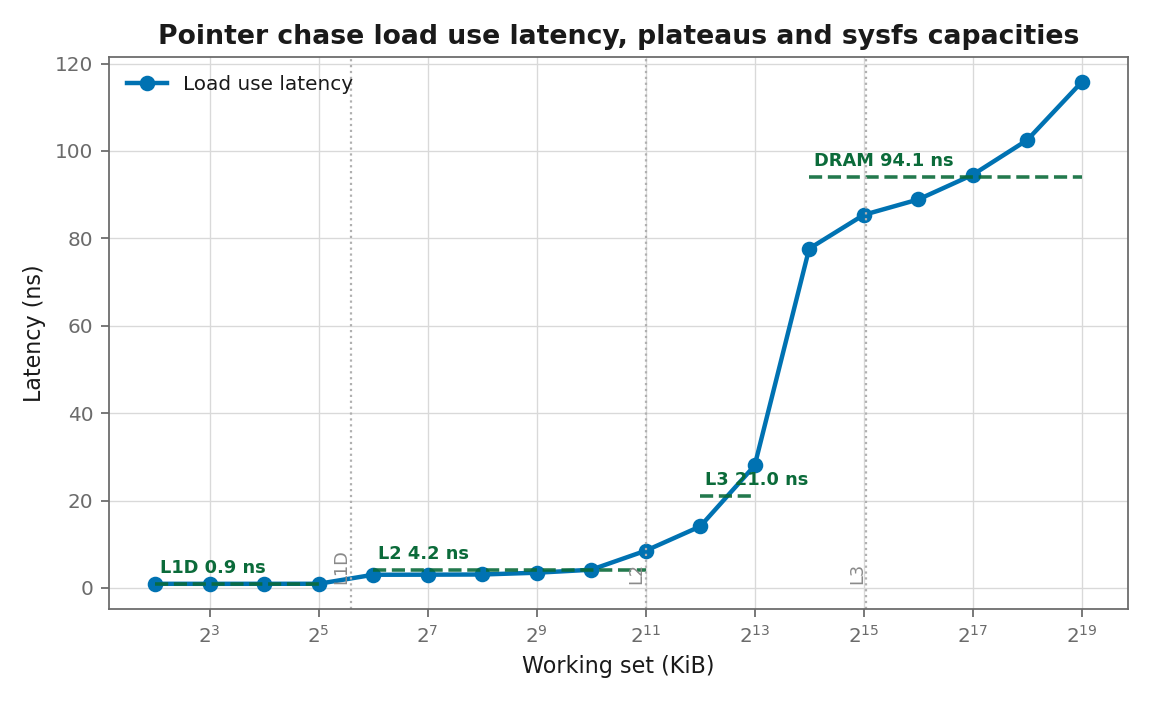
\includegraphics[width=\linewidth]{latency_plateau.png}
\caption{Load use latency against working set, with detected plateau means and
the sysfs cache capacities marked. The step to DRAM begins about one octave
below the nominal 33 MB L3, an effect of TLB reach and associativity under
random access.}
\label{fig:latency}
\end{figure}

\begin{table}[h]
\centering
\caption{Detected latency plateaus, cross checked against sysfs.}
\label{tab:latency}
\begin{tabular}{llrr}
\hline
Region & Working set & Latency (ns) & Cycles \\
\hline
L1D & 4 to 32 KiB & 0.94 & 5.0 \\
L2 & 64 to 2048 KiB & 4.29 & 22.9 \\
L3 & 4096 to 8192 KiB & 20.03 & 107.0 \\
DRAM & 16384 to 524288 KiB & 93.38 & 498.8 \\
\hline
\end{tabular}

\end{table}

The change point detector places the L1 boundary within \num{0.08} octaves of
the 48 KB L1 capacity and the L2 boundary within \num{0.50} octaves of the 2 MB
L2. The DRAM onset is flagged about \num{1.5} octaves below the nominal L3
capacity, which the discussion addresses.

\section{Bandwidth}

Single thread bandwidth by variant is in Table~\ref{tab:bandwidth} and
Figure~\ref{fig:variants}. The non temporal variant wins on Add and Triad, where
avoiding the read for ownership pays off, while the scalar and vectorized
variants are competitive on Copy. The thread scaling curve
(Figure~\ref{fig:scaling}) saturates near \SI{78}{\giga\byte\per\second} by four
to five threads, about 87 percent of the DDR5-5600 dual channel theoretical
\SI{89.6}{\giga\byte\per\second}. Beyond that point additional P cores, and then
the E cores, add no bandwidth: the reported knee is the bandwidth wall, not a P
to E transition.

\begin{table}[h]
\centering
\caption{Single thread STREAM bandwidth by variant, GB/s.}
\label{tab:bandwidth}
\begin{tabular}{lrrrr}
\hline
Variant & Copy & Scale & Add & Triad \\
\hline
Scalar & 43.9 & 23.1 & 27.1 & 28.7 \\
Auto vectorized & 46.1 & 26.3 & 31.8 & 31.4 \\
AVX2 NT stores & 36.7 & 36.8 & 41.3 & 40.8 \\
\hline
\end{tabular}

\end{table}

\begin{figure}[h]
\centering
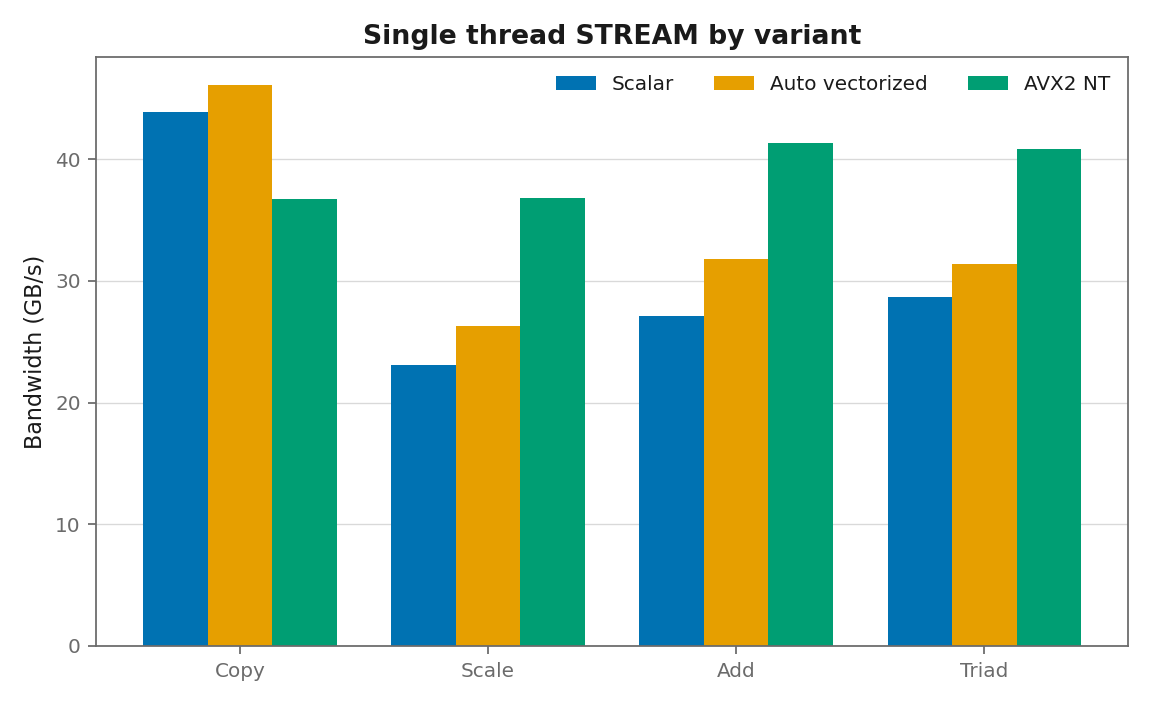
\includegraphics[width=0.85\linewidth]{variant_comparison.png}
\caption{Single thread bandwidth by kernel and variant.}
\label{fig:variants}
\end{figure}

\begin{figure}[h]
\centering
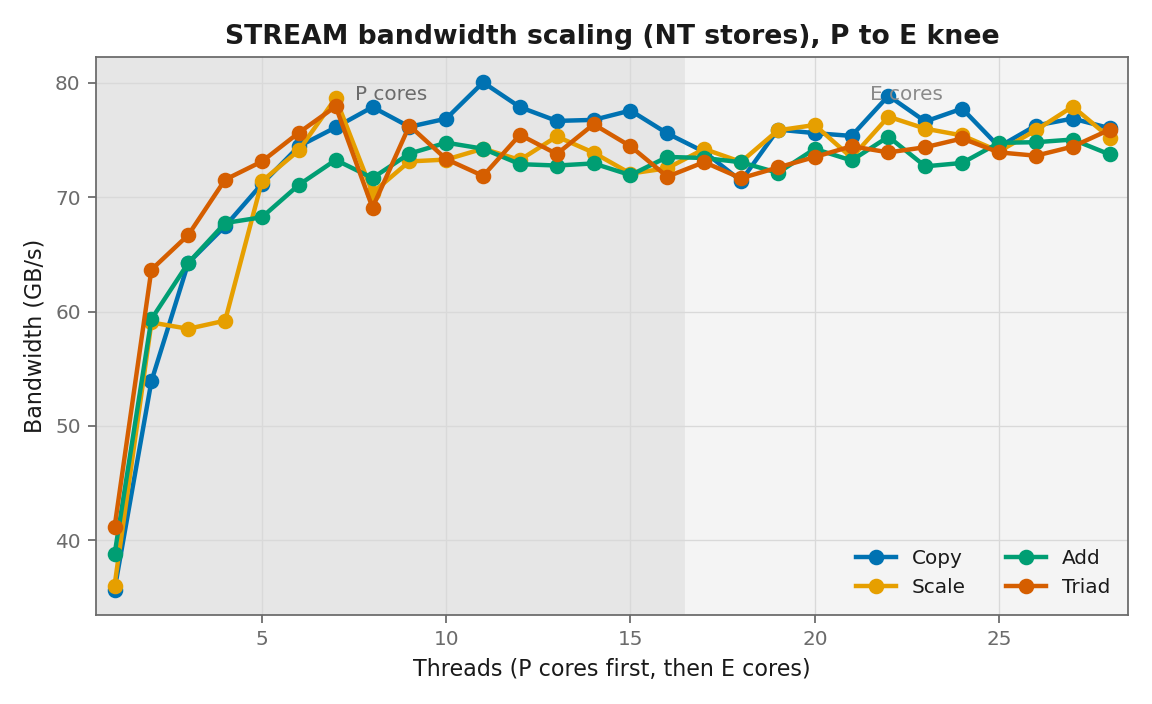
\includegraphics[width=0.85\linewidth]{bandwidth_scaling.png}
\caption{Bandwidth scaling, P cores first then E cores. The curve saturates well
before the cores are exhausted.}
\label{fig:scaling}
\end{figure}

\section{Peak FLOPS}

Table~\ref{tab:flops} compares measured throughput to the ceiling computed from
the same measured clock. One P core reaches about \SI{170}{GFLOPS}, which is 99
percent of its ceiling; matching the ceiling to within one percent is the
expected result for a saturating ten chain loop and confirms both the clock and
the FLOP counting. All 28 logical CPUs together reach about \SI{1900}{GFLOPS}.

\begin{table}[h]
\centering
\caption{Peak single precision throughput against the computed ceiling.}
\label{tab:flops}
\begin{tabular}{lrrr}
\hline
Configuration & GFLOPS & Ceiling & Efficiency \\
\hline
Single P core & 169.7 & 172.4 & 98\% \\
All core (28 threads) & 1878 & (aggregate) & \\
\hline
\end{tabular}

\end{table}

\section{Roofline and tile prediction}

Figure~\ref{fig:roofline} places the suite's kernels on the measured roofline.
STREAM Triad sits on the memory bound slope. The single core FMA loop sits on the
single core ceiling. The naive blocked GEMM, though high in arithmetic intensity
and therefore compute bound in principle, sits well below the single core
ceiling: the gap is the cost of not packing.

Table~\ref{tab:tile} compares the BLIS analytical tile prediction to the
empirical best from the GEMM sweep. They disagree: the model predicts a large
$K_c$, the naive kernel prefers a much smaller one. This miss is a finding, not a
failure, and the discussion explains it.

\begin{figure}[h]
\centering
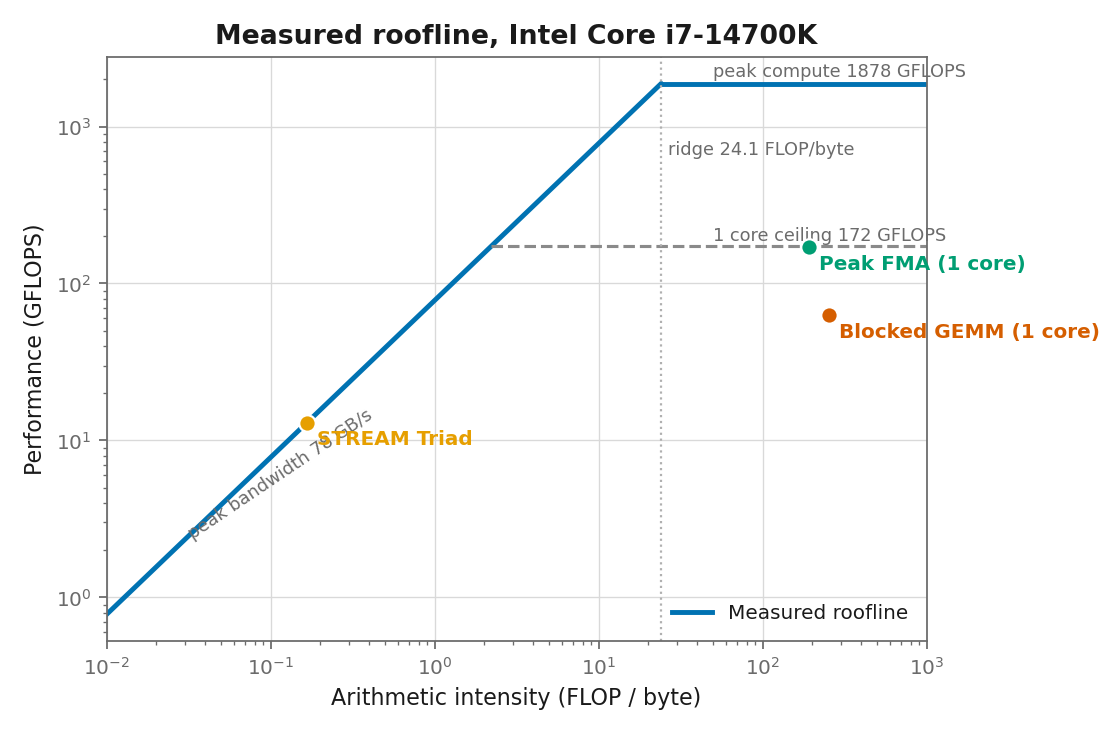
\includegraphics[width=\linewidth]{roofline.png}
\caption{Measured roofline with all core and single core compute ceilings.}
\label{fig:roofline}
\end{figure}

\begin{table}[h]
\centering
\caption{BLIS analytical prediction versus empirical best tile.}
\label{tab:tile}
\begin{tabular}{lrrr}
\hline
Source & Mc & Kc & Nc \\
\hline
BLIS analytical & 704 & 696 & 11296 \\
Empirical best & 384 & 64 & 1536 \\
\hline
\end{tabular}
% Kc prediction is a miss of 3.4 octaves in Kc.

\end{table}

\chapter{Discussion}

\section{The DRAM onset below nominal L3}

The latency staircase steps up to DRAM near an 8 to 16 MB working set, while the
L3 is 33 MB. Single threaded random pointer chasing does not reach the full L3
before latency climbs, because the random 64 byte stride thrashes the
translation lookaside buffer, whose reach with 4 KB pages is limited, and it
stresses L3 associativity and replacement. Effective capacity under this access
pattern is roughly half the nominal size. This is expected
behavior~\cite{drepper2007}, and the sysfs cross check is designed to flag it
rather than smooth it away. Large pages would isolate a purer DRAM latency, at
the cost of measuring something less representative of ordinary code.

\section{The bandwidth wall}

Bandwidth saturates at four to five threads. This is the defining feature of a
memory bound workload on a dual channel desktop: the DRAM channels are the
bottleneck, and once they are full, more cores cannot help. The practical
consequence is that the P versus E core question is moot for STREAM, since the
knee arrives long before the core count does. It would matter for a compute
bound workload, where the E cores add throughput, which is visible in the all
core FLOPS number.

\section{Why the tile prediction misses}

The BLIS analytical model assumes a packed micro kernel in which the L1 resident
panel of $B$ is only $N_r$ elements wide. The validation kernel here is
deliberately naive: it does not pack, and its inner loop spans the full width of
$B$. Each reused row of $B$ is therefore the full matrix width, several
kilobytes, so only a handful of rows fit in L1 or L2 at once, and the optimum
moves to a much smaller $K_c$ than the packed model wants. The prediction is not
wrong for the kernel it describes; it is describing a different kernel. Closing
the gap means implementing the packed micro kernel the model assumes, which is
the natural next step and is recorded as future work.

\section{Limitations}

The clock is measured in software, not read from a counter, so it carries a few
percent of uncertainty; this is why efficiencies are reported as approximate and
a match to within one percent is treated as confirmation rather than a precise
claim. Bandwidth uses float arrays and the classical STREAM byte convention. The
hybrid P and E identification is heuristic under WSL2. None of these affect the
qualitative conclusions, and each is stated where it applies.

\chapter{Conclusion}

Every headline number a specification sheet quotes for this class of processor
was measured directly and cross checked. The cache latencies recover the L1, L2,
L3, and DRAM plateaus and agree with the Raptor Cove figures in cycles once the
clock is measured honestly. Sustainable bandwidth reaches 87 percent of the
theoretical dual channel peak and saturates at four to five threads, exposing
the bandwidth wall. Peak single precision throughput matches the ceiling
computed from the same measured clock to within one percent. The ceilings form a
roofline on which the suite's own kernels sit exactly where the model predicts,
and a BLIS style tile prediction, tested against a blocked GEMM sweep, misses the
naive kernel in a way that is fully explained by the absence of packing.

The recurring lesson is that the platform, not the arithmetic, is where the
honesty is won or lost. On WSL2 the reported clock ignores turbo and the hybrid
topology is hidden, and each of these, left unexamined, would have produced a
confidently wrong table. Measuring the clock in software and flagging the
heuristic topology turned both into stated, understood conditions. The natural
continuation is a packed GEMM micro kernel that would close the roofline gap and
let the tile prediction be tested against a kernel built on the same assumptions.


\bibliographystyle{plain}
\bibliography{refs}

\end{document}
